\documentclass{beamer}
\usetheme{Warsaw}

\usepackage[utf8]{inputenc}
\usepackage{fancybox}
\usepackage{multimedia} 
\usepackage{subfig}
\usepackage{amsmath}
\usepackage{hyperref}
\usepackage[all]{xy}
\begin{document}


\title[Stochastik] % (optional, only for long titles)
{Wahrscheinlichkeitstheorie und Statistik (Stochastik)
\\
\includegraphics[scale=0.5]{img/craps}
}
\subtitle{}
\author[Dr. Johannes Riesterer] % (optional, for multiple authors)
{Dr.  rer. nat. Johannes Riesterer}

\date[KPT 2004] % (optional)
{}

\subject{Stochastik}

\frame{\titlepage}

\begin{frame}
    \frametitle{Einleitung}
\framesubtitle{Was ist Stochastik?}
    \begin{block}{Wahrscheinlichkeitstheorie}
 Beschreibung und Untersuchung von zufälligen Vorgängen und Modellen.
\end{block}
    \begin{block}{Statistik}
Umgang mit dem Zufall und Schlussfolgern aus Beobachtungen
\end{block}
 \end{frame}

\begin{frame}
    \frametitle{Einleitung}
\framesubtitle{}
    \begin{block}{Mathematik und Realität}

\begin{figure}[htp]
      \centering
    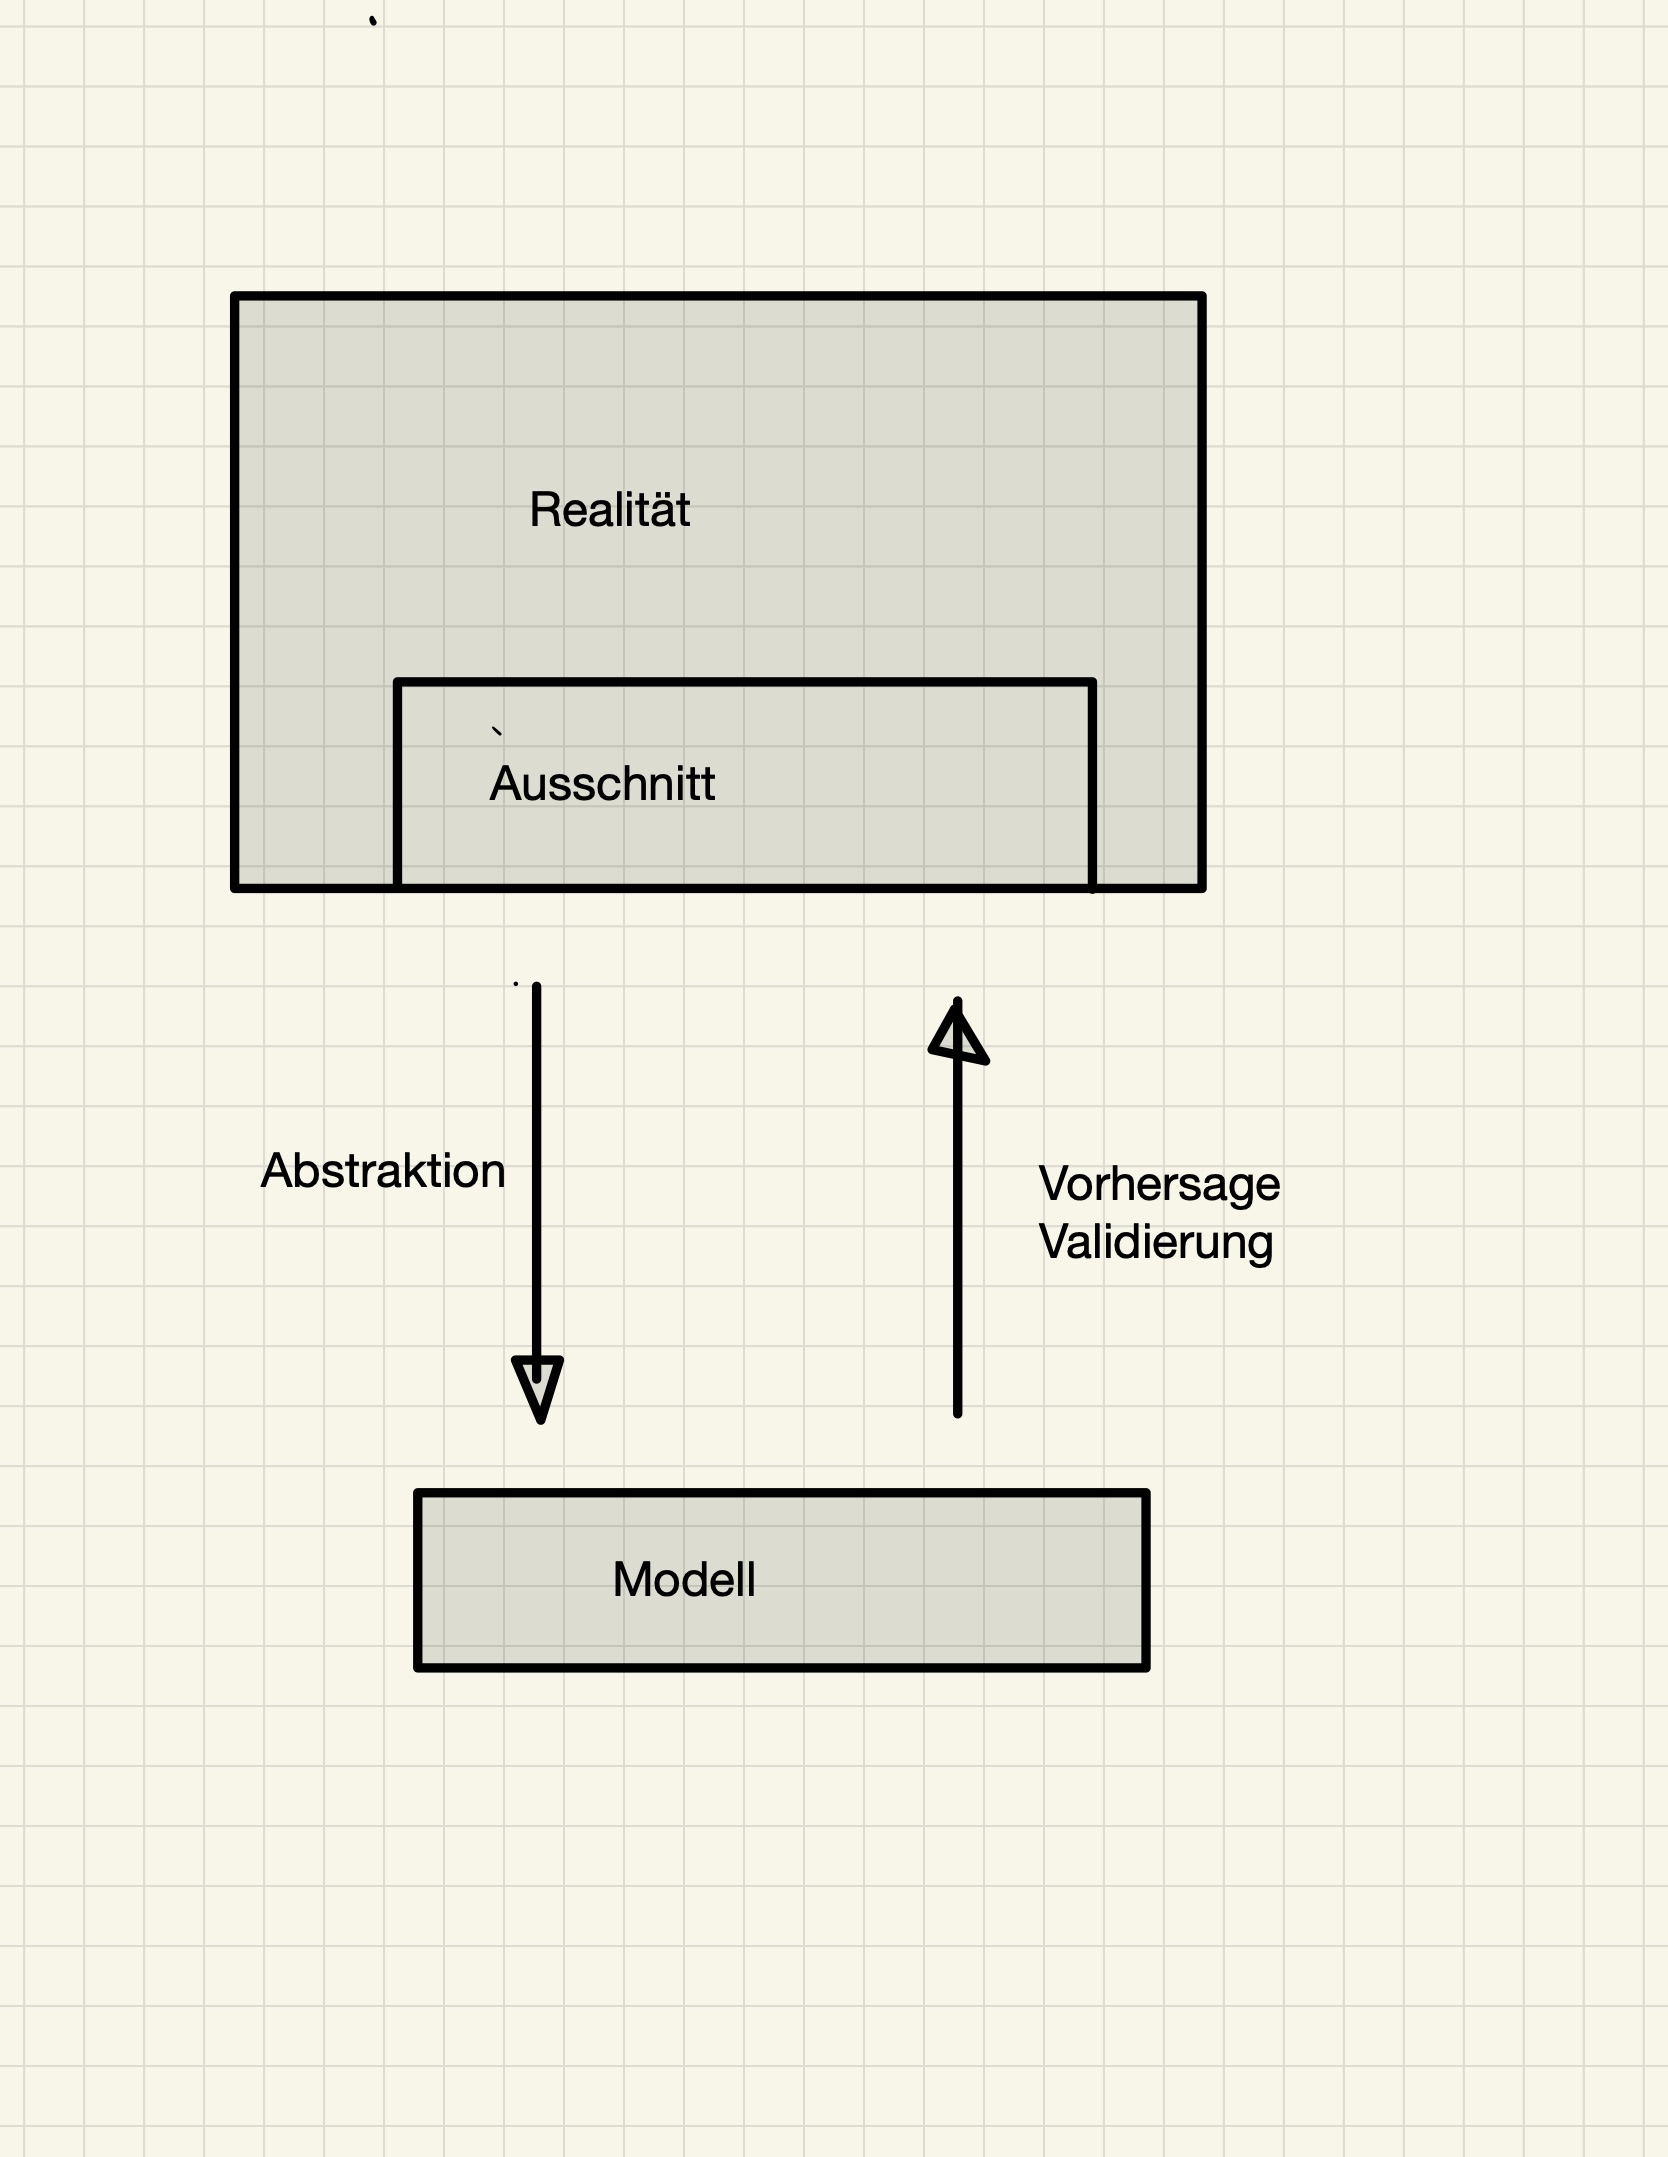
\includegraphics[width=0.5 \textwidth]{img/modellierung}

 
\end{figure}
\end{block}
 
 \end{frame}


\begin{frame}
    \frametitle{Einleitung}
\framesubtitle{}

    \begin{block}{Was ist Zufall}
Keine kausale Erklärung für den Ausgang eines Vorganges vorhanden (Nicht-Deterministisch)
\end{block}



   \begin{block}{Kausalität (Wikipedia)}
Kausalität ist die Beziehung zwischen Ursache und Wirkung. Sie betrifft die Abfolge von Ereignissen und Zuständen, die aufeinander bezogen sind. Demnach ist A die Ursache für die Wirkung B, wenn B von A herbeigeführt wird.
\end{block}

\begin{figure}[htp]
      \centering
    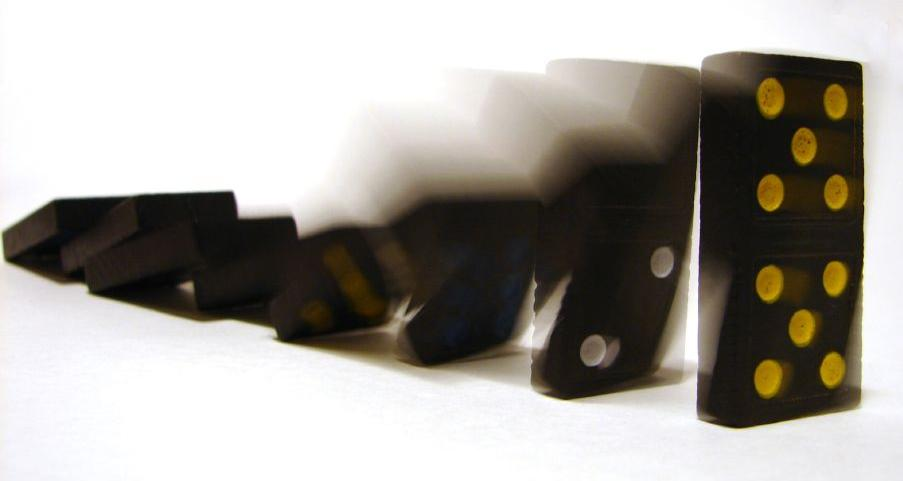
\includegraphics[width=0.3\textwidth]{img/Domino}

      \caption{Quelle: Wikipedia}
\end{figure}


\end{frame}


\begin{frame}
    \frametitle{Einleitung}
\framesubtitle{}
   \begin{block}{Stochastik vs. Kausalität}
In den seltensten Fällen lassen sich aus stochastischen Zusammenhängen kausale Zusammenhänge ableiten. ACHTUNG: Populisten tun dies jedoch ständig!
\end{block}

\end{frame}


\begin{frame}
    \frametitle{Einleitung}
\framesubtitle{}

    \begin{block}{Stochastik vs. Kausalität}
Beobachtung: Bei Regen tragen die Menschen einen Regenschirm.
Es folgt NICHT: Wenn man einen Regenschirm aufspannt, fängt es an zu regnen.
Ebenso folgt NICHT: Wenn es regnet, sieht man Menschen mit Regenschirmen. 
\end{block}


\begin{figure}[htp]
      \centering
    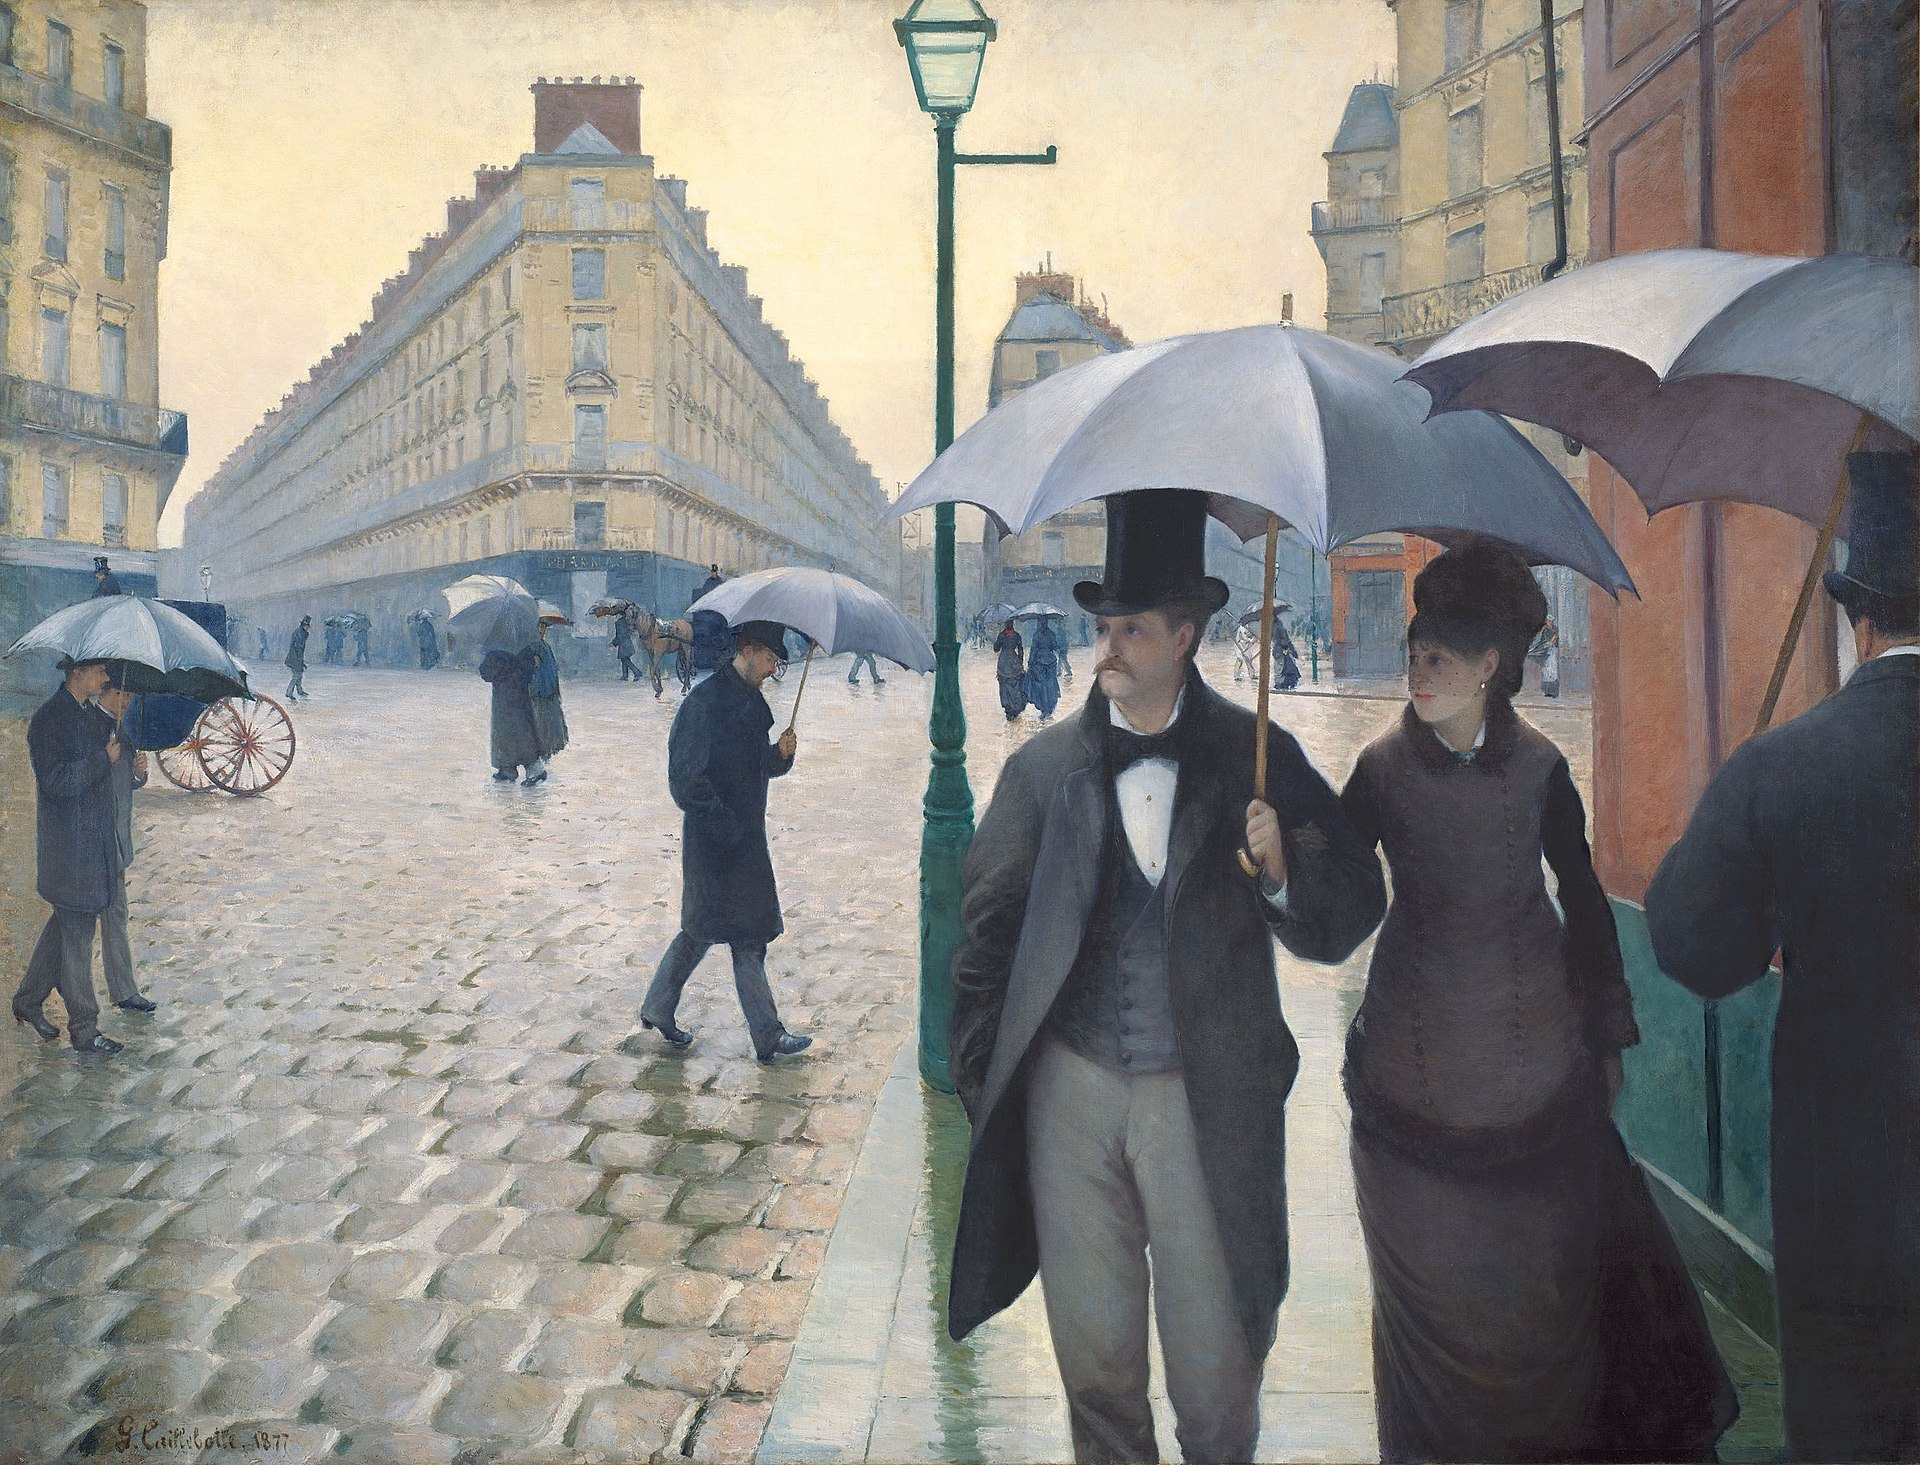
\includegraphics[width=0.6\textwidth]{img/Paris}

      \caption{Quelle: Wikipedia}
\end{figure}


\end{frame}




\begin{frame}
    \frametitle{Einleitung}
\framesubtitle{}
\begin{block}{}
Gibt es überhaupt Zufall? 
\end{block}

\begin{figure}[htp]
      \centering
    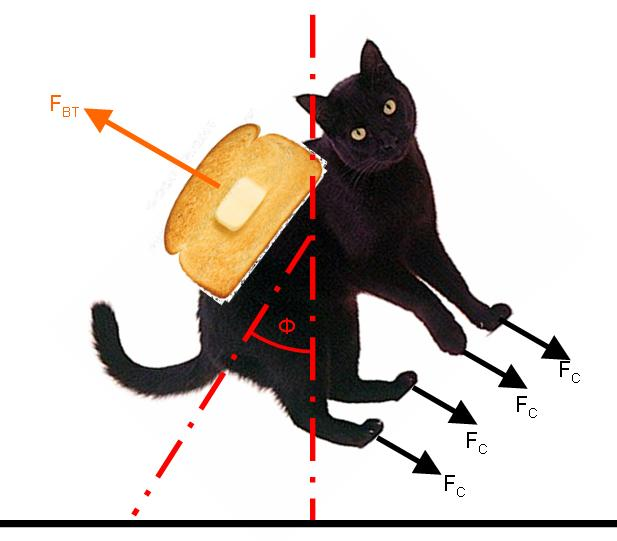
\includegraphics[width=0.2\textwidth]{img/katze-toast}

      \caption{Quelle: https://www.laurentinews.de/wp-content/uploads/2014/03/katze-toast1.jpg}
\end{figure}

    \begin{block}{}
Zufall hängt von der betrachteten Skala ab. \\
Physik $\Rightarrow$ Skalen können nicht beliebig klein werden.
\end{block}
    \begin{block}{}
\href{https://de.wikipedia.org/wiki/Brownsche_Bewegung
}{Wikipedia://Brownsche Molekularbewegung.
}
\end{block}

\end{frame}



\begin{frame}
    \frametitle{Einleitung}
\framesubtitle{}

\begin{block}{Motivation}
Maschinelles Lernen. Maschinelle Vorhersage. Informationstheorie. Prozesstheorie. Optimierungstheorie. Mustererkennung. Komplexitätstheorie, bildgebende Verfahren, Physik.
\end{block}

\begin{block}{Motivation}

Wie programmiere und trainiere ich einen "intelligenten" Spam-Filter?
Ab wie vielen richtig beantworteten Ja-Nein-Fragen ist der  von meinem Kommilitonen gebaute Roboter wirklich intelligent und  hat nicht nur zufällig die richige Antwort gewählt?
Wie bewertet Google Webseiten?
Warum wird das Rauschen von Sensoren ständig als Normalverteilt angenommen?
Macht es Sinn auf Rot zu setzen, nachdem 100 mal Schwarz im Roulette fiel?
Kann man Geschwafel quantifizieren?
Wie kann man mit einer Münze Integrale lösen und was hat das mit Hollywood zu tun? 
\end{block}

 \end{frame}

\begin{frame}
    \frametitle{Einleitung}
\framesubtitle{}

\begin{block}{Literatur}
\begin{itemize}
\item Stochastik für Informatiker; L. Dümbgen; Springer
\item Einführung in die Wahrscheinlichkeitstheorie und Statistik; Hans-Otto Georgii; De Gruyter Studium
\item Achim Klenke; Wahrscheinlichkeitstheorie; Springer
\end{itemize}
\end{block}


 \end{frame}



\begin{frame}
    \frametitle{Highlight}
\framesubtitle{}
\begin{figure}[htp]
      \centering
    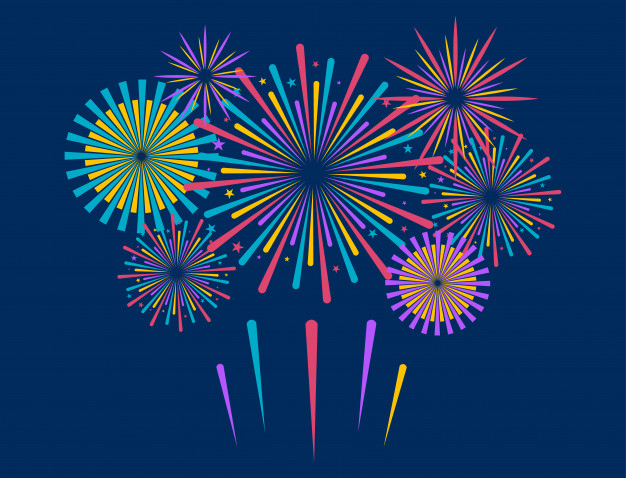
\includegraphics[width=0.9\textwidth]{img/firework}
\end{figure}
 \end{frame}


\begin{frame}
    \frametitle{Einleitung}
\framesubtitle{}

\begin{block}{Bessere Entscheidungen durch Mathematik?!?}
Gegeben sind 3 geschlossene Türen.  Hinter einer ist der Hauptgewinn, hinter zwei eine Ziege.
Der Spieler darf  sich zuerst für eine Tür entscheiden. 
Danach öffnet der Moderator eine der  nicht gewählten Türen, hinter der nicht der Hauptgewinn ist und fragt den Spieler, oben er seine vorige Entscheidung revidieren und die andere geschlossene Tür öffnen möchte.
\end{block}

\begin{figure}[htp]
      \centering
    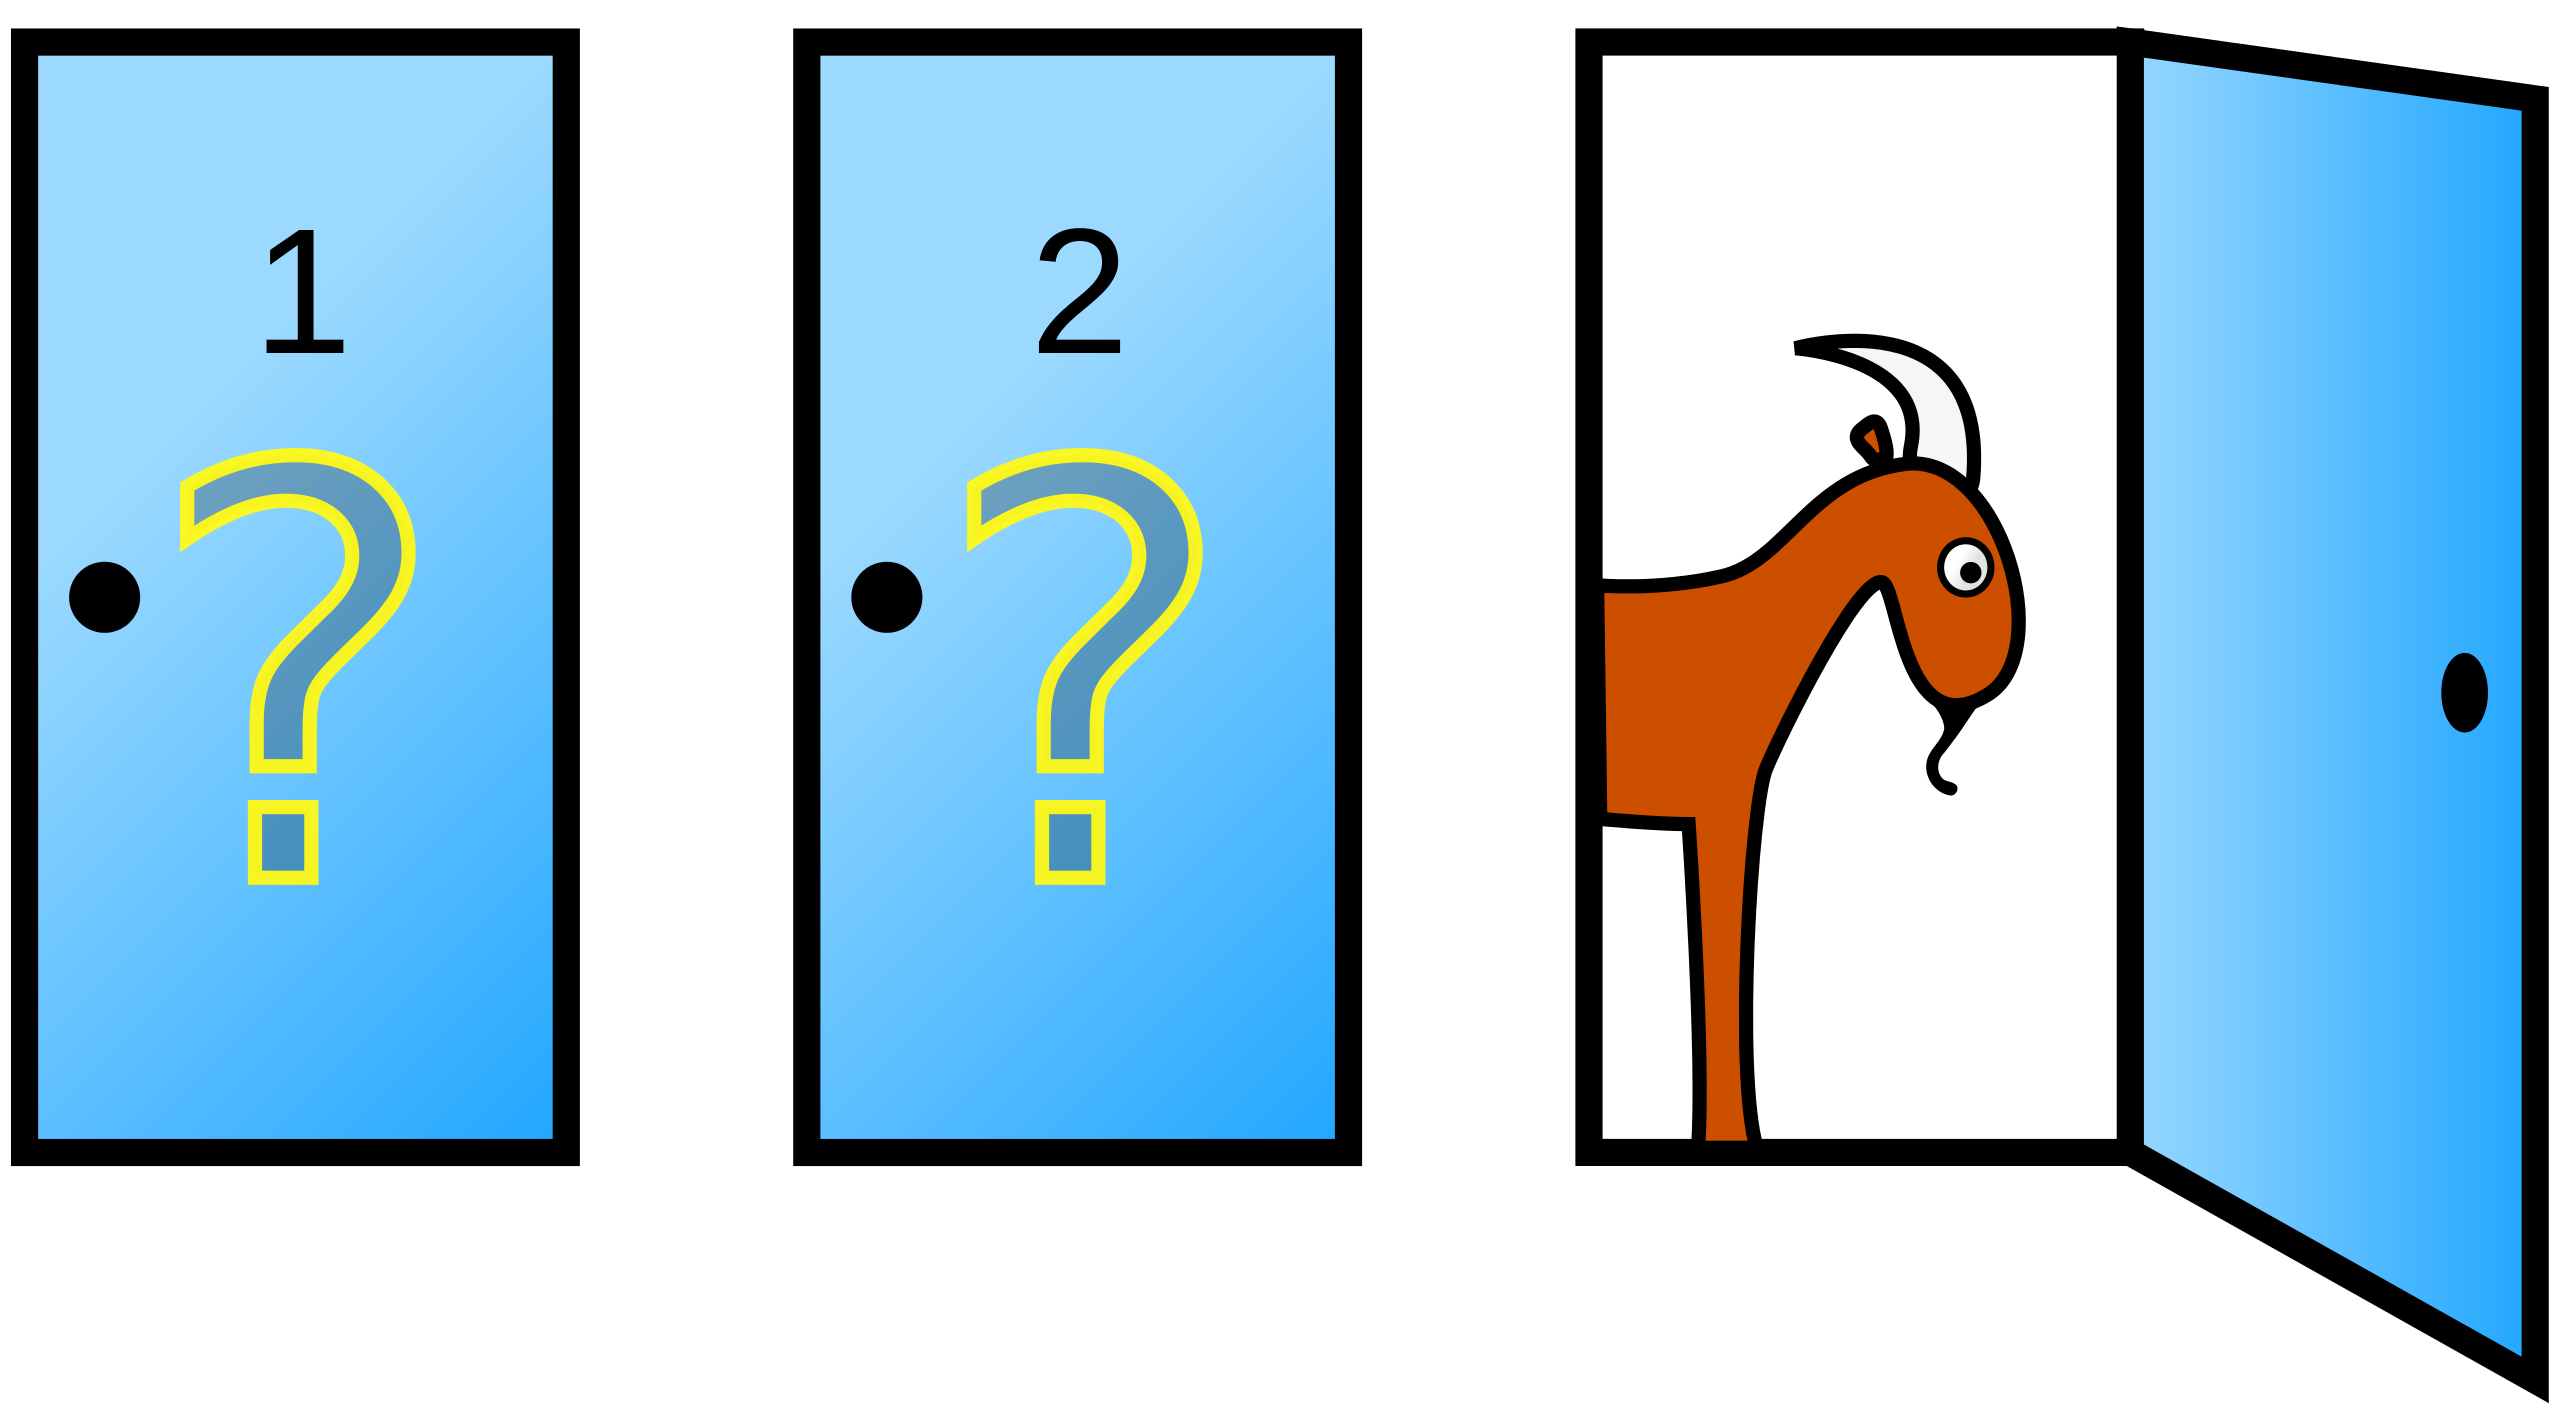
\includegraphics[width=0.45\textwidth]{img/Monty_open}

      \caption{Quelle: Wikipedia}
\end{figure}

 \end{frame}

\begin{frame}
    \frametitle{Einleitung}
\framesubtitle{}

\begin{block}{Bessere Entscheidungen durch Mathematik?!?}
Hat der Spieler eine höhere Gewinnchance, wenn er die Tür wechselt?
\end{block}

 \end{frame}

\begin{frame}
    \frametitle{Einleitung}
\framesubtitle{}

\begin{block}{Bessere Entscheidungen durch Mathematik?!?}
Wechseln hat eine höhere Gewinnchance!
\end{block}

\begin{figure}[htp]
      \centering
    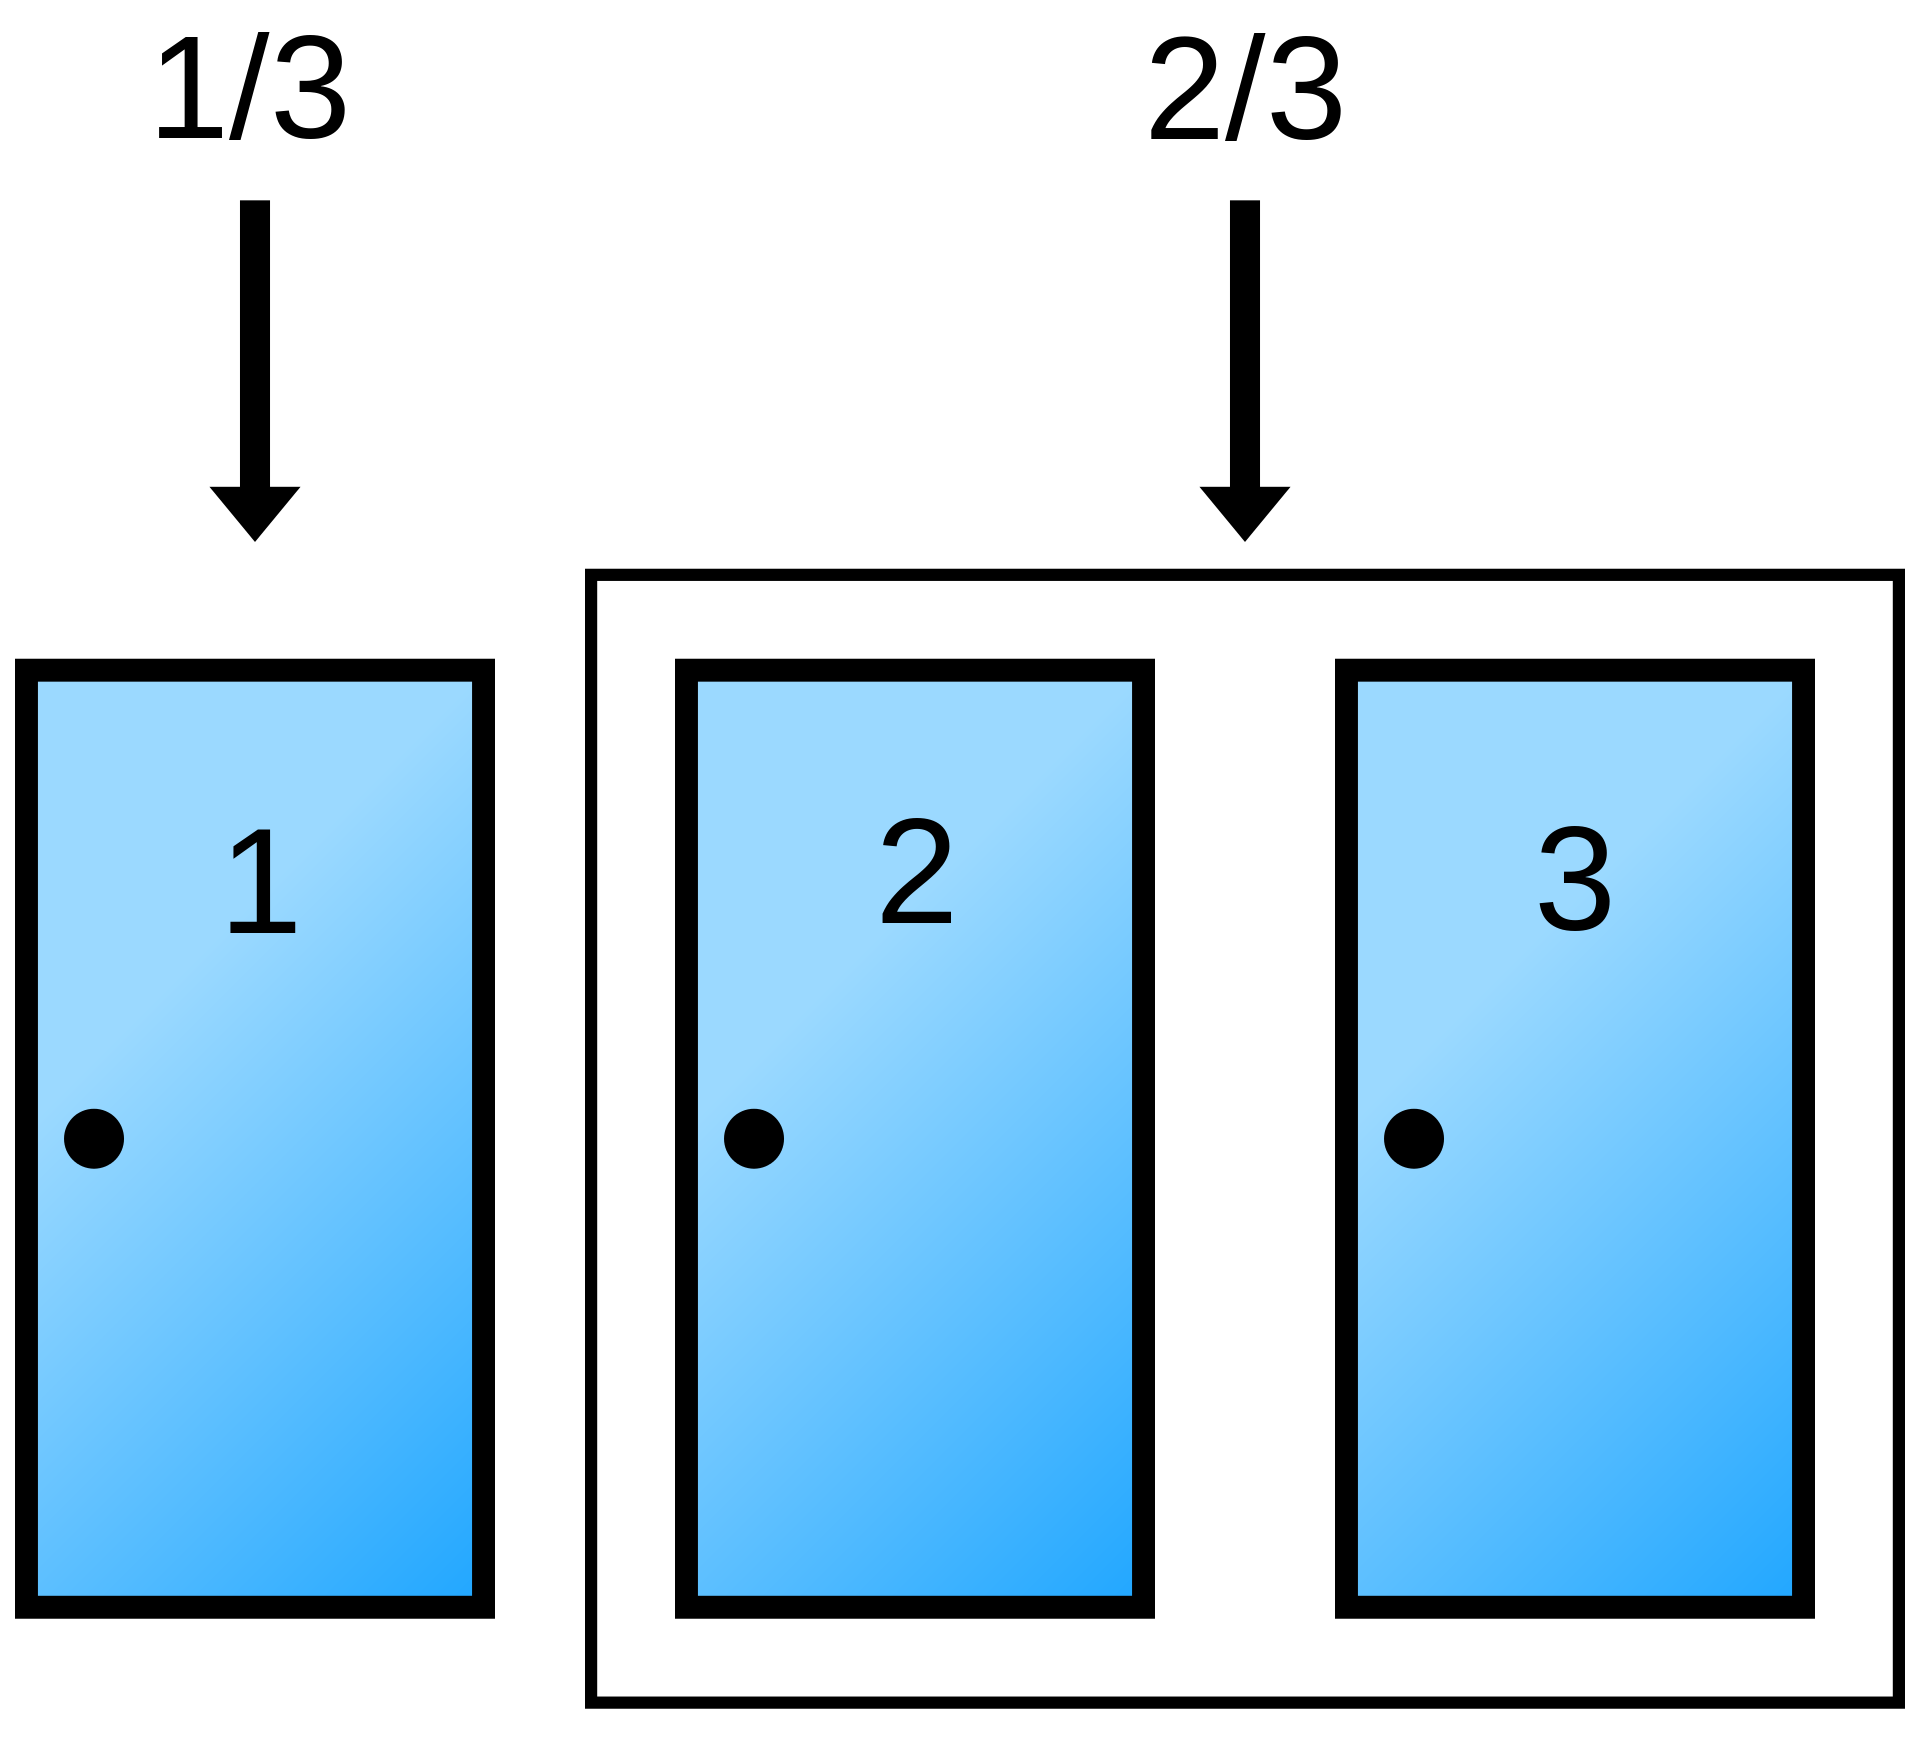
\includegraphics[width=0.45\textwidth]{img/Monty_closed_1}
    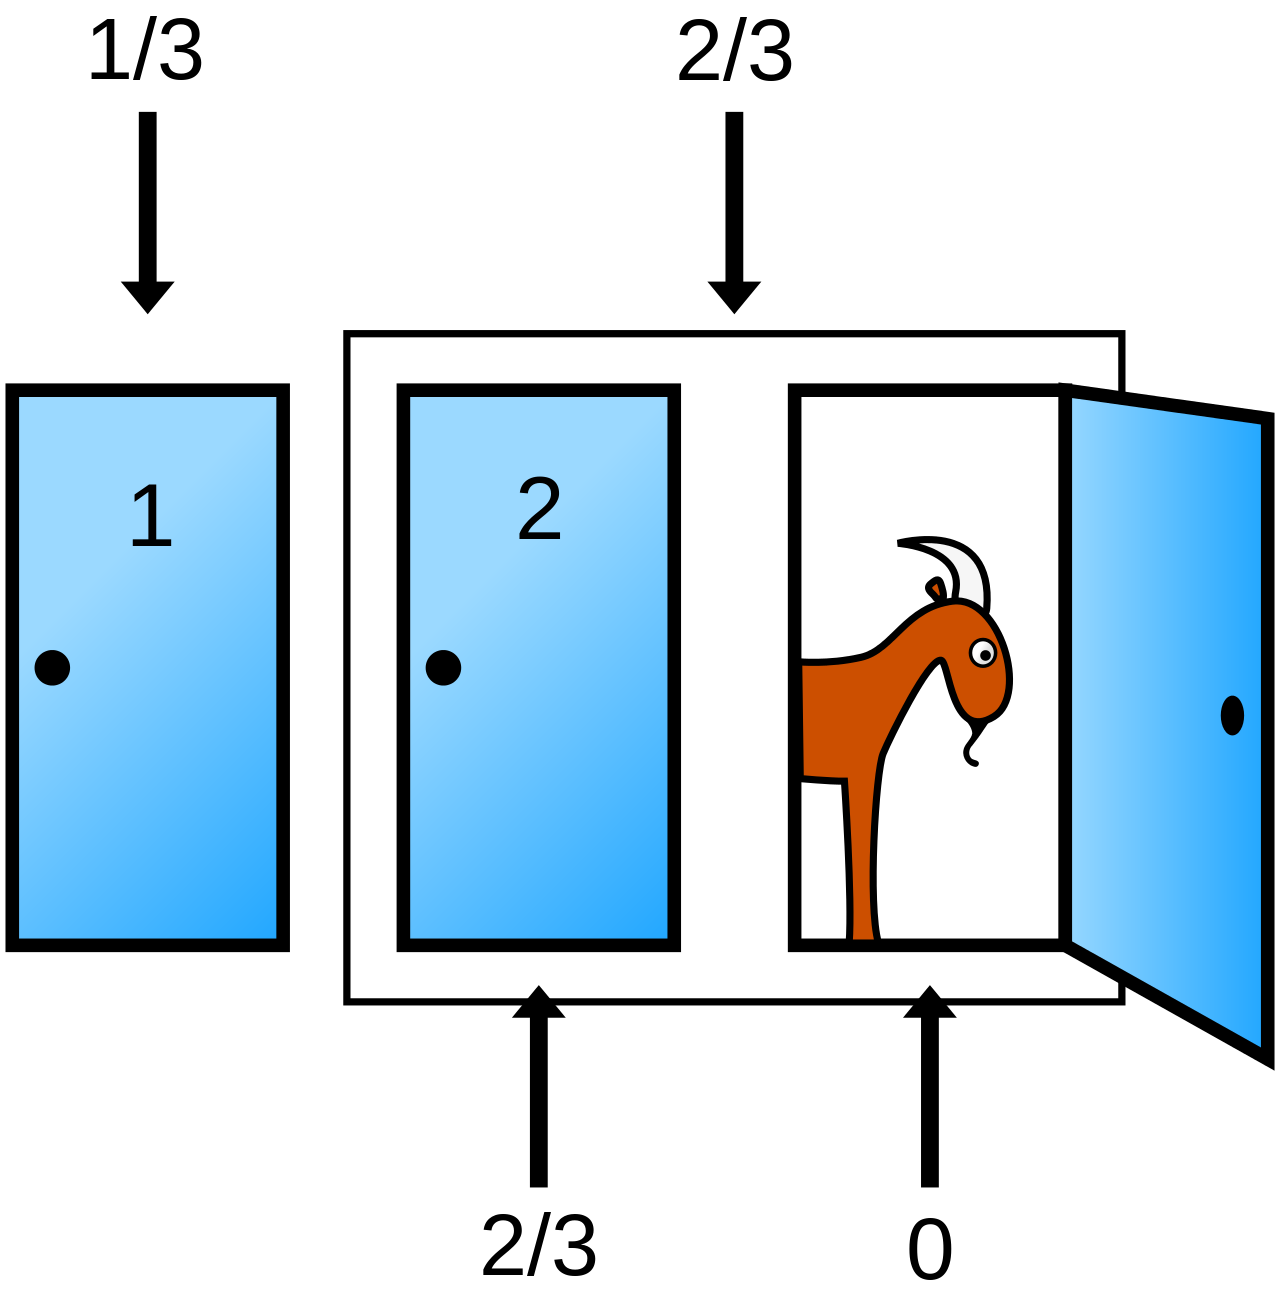
\includegraphics[width=0.45\textwidth]{img/Monty_open_1}
      \caption{Quelle: Wikipedia}
\end{figure}

 \end{frame}


\begin{frame}
    \frametitle{Diskrete Modelle}
\framesubtitle{ Laplace Wahrscheinlichkeit}

\begin{block}{Laplace Wahrscheinlichkeit}
Gegeben endliche Menge $\Omega$ (Grundmenge). \\
Potenzmenge  $\mathcal{P}(\Omega)$   (Menge aller Teilmengen).  \\
$A \in \mathcal{P}(\Omega)$ bezeichnet man auch als Ereignis. 
\begin{align*}
& P(A) := \frac{ \#A}{ \# \Omega} \\
 & (\#M := \text{Anzahl der Elemente von M})
\end{align*}
heißt Laplace Wahrscheinlichkeit.
\end{block}

\begin{block}{Komplementäres Ereignis}
\begin{align*}
& P(A^c) := P(\bar{A}) := 1 - P(A)
 & A^c := \{ \omega \in \Omega | \omega \notin A \}
\end{align*}
\end{block}


 \end{frame}
 
 \begin{frame}
    \frametitle{Diskrete Modelle}
\framesubtitle{ Laplace Wahrscheinlichkeit}

\begin{block}{Beispiel (Würfel)}
Für einen einmaligen Wurf eines Würfels sei $\Omega := \{1,2,3,4,5,6\}$. \\
Ein mögliches Ereignis $A \in \mathcal{P}(\Omega)$ wäre das Ereignis $A := \{3,4\}$, also das Ereignis eine 3 oder eine 4 zu würfeln.  \\
Hierzu ist die Laplace Wahrscheinlichkeit dann 
\begin{align*}
& P(A) = \frac{ \#A}{ \# \Omega} = \frac{2}{6}
\end{align*}
Das Gegenereignis hierzu ist $A^c = \{1,2,5,6\}$ mit $P(A^c) = \frac{4}{6}$
\end{block}

 \end{frame}



\begin{frame}
    \frametitle{Diskrete Modelle}
\framesubtitle{Kombinatorik}
\begin{block}{Variationen und Kombinationen}

Sei $n = \#\Omega$ und $k \leq n$.
\begin{itemize}
\item $Var_k^n(\Omega, m.W.) : = \{ ( \omega_1, \ldots, \omega_k) \ |\  \omega_i \in \Omega \}$  Menge aller Variationen mit Wiederholung.
\item $Var_k^n(\Omega, o.W.) : = \{ ( \omega_1, \ldots, \omega_k) \ |\  \omega_i \in \Omega; \;  \omega_i \neq \omega_j  \}$  Menge aller Variationen ohne Wiederholung.
\item $Kom_k^n(\Omega, m.W.) : = \{ ( \omega_{i_1}, \ldots, \omega_{i_k})  \ |\  \omega_{i_l} \in \Omega; \; 1  \leq i_1 \leq  \ldots  \leq i_k  \}$  Menge aller Kombinationen  mit Wiederholung.
\item $Kom_k^n(\Omega, o.W.) : = \{ ( \omega_{i_1}, \ldots, \omega_{i_k} ) \ |\  \omega_{i_l} \in \Omega; \; 1 \leq i_1  \leq \ldots \leq i_k; \;  \omega_{i_i} \neq \omega_{i_j} \} $  Menge aller Kombinationen  ohne  Wiederholung.
\end{itemize}
\href{https://de.wikipedia.org/wiki/Tupel}{Notation geändert. Vergleiche Tupel auf Wikipedia}
\end{block}

 \end{frame}
 
\begin{frame}
    \frametitle{Diskrete Modelle}
\framesubtitle{Kombinatorik}

\begin{block}{Beispiel (Würfel)}
\begin{itemize}
\item Das Tupel $ (3,3,2,5 )  \in Var_4^6(\Omega, m.W.)$ ist eine mögliche Variation mit Wiederholung.
\item Das Tupel $ (4,2,1,5 ) \in Var_4^6(\Omega, o.W.)$ ist eine mögliche Variation ohne Wiederholung.
\item Das Tupel $ (2,3,3,5 )  \in Kom_4^6(\Omega, m.W.)$ ist eine mögliche Kombination mit Wiederholung.
\item Das Tupel $(1,2,4,5) \in Kom_4^6(\Omega, o.W.)$ ist eine mögliche Kombination ohne Wiederholung.

\end{itemize}

\end{block}
 \end{frame}



\begin{frame}
    \frametitle{Diskrete Modelle}
\framesubtitle{Kombinatorik}

\begin{block}{Variationen und Kombinationen}
\begin{itemize}
\item $\# Var_k^n(\Omega, m.W.)  = n^k = \underbrace{n \cdot n \cdots n}_{\text{k-mal}}$
\item $\# Var_k^n(\Omega, o.W.)  = n_k = n \cdot (n-1) \cdots  (n-k+1) = \frac{n!}{(n-k)!}$  
\item $\#Kom_k^n(\Omega, o.W.) = \binom{n}{k} = \frac{n!}{k! (n-k)!}$  
\item $\#Kom_k^n(\Omega, m.W.)  = \binom{n + k -1}{k}$  
\end{itemize}
\end{block}
 \end{frame}




\end{document}
